\documentclass{beamer}
% Load csquotes for the \enquote command
\usepackage{csquotes}
\usepackage{hyperref}
% Load biblatex for bibliography management
\usepackage[backend=biber, style=authoryear]{biblatex}
\addbibresource{bibliography.bib} % Specify your BibTeX bibliography file

\mode<presentation> {
\usetheme{CambridgeUS}
\usecolortheme{seahorse}
}

\title{Macroéconomie 1}
\author{Mart\'in Valdez}
\date{IE1}

\begin{document}

\begin{frame}
\titlepage
\end{frame}

\begin{frame}
\frametitle{Overview}
\tableofcontents
\end{frame}

% Slide Template
\section{Introduction}
\begin{frame}
\frametitle{Introduction}
\begin{itemize}
    \item Course Overview
    \item Objectives
    \item Grading
\end{itemize}
\end{frame}

\section{Economic Concepts}
\begin{frame}
\frametitle{Micro vs. Macro}
\begin{itemize}
    \item \textbf{Microéconomie}
    L'étude des agents économiques individuels tels que les ménages et les entreprises,
    comment ils prennent des décisions, et comment ils interagissent dans les marchés individuels.
    \pause
    \item \textbf{Macroéconomie}
    L'étude de l'économie dans son ensemble, incluant des mesures globales telles que
    le PIB, la consommation, l'investissement, l'inflation et le chômage.
    \begin{itemize}
        \item \textbf{Short-run(Court terme) :} Cycles économiques, récessions, et politiques monétaires et fiscales.\pause
        \item \textbf{Long-run(Long terme) :} Croissance économique, productivité et commerce international.
    \end{itemize}
\end{itemize}
\end{frame}

\begin{frame}
    \frametitle{Micro vs. Macro}
    \textbf{Pourquoi étudier la macroéconomie ?}
    \begin{itemize}\pause
        \item \textbf{C'est important :} 
        La macroéconomie a un impact direct sur la vie des gens.\pause
        \item \textbf{C'est utile :} Politiciens ont en besoin pour 
        prendre des décisions éclairées sur les politiques économiques.\pause
        \item \textbf{Responsabilité sociale :} Comprendre les politiques économiques.
    \end{itemize}
    \end{frame}
    
    

%------------------------------------------------
%  History of Macroeconomics
%------------------------------------------------
\begin{frame}
    \frametitle{Histoire de la Macroéconomie}
    \framesubtitle{Pré-critique de Lucas : 1936-1976}
        \begin{itemize}
            \item Le livre fondateur de John Maynard Keynes en 1936, \enquote{Théorie générale de l'emploi, de l'intérêt et de la monnaie}
            \item \textbf{Économie keynésienne :} Prône l'intervention gouvernementale pour stabiliser l'économie.
            \item \textbf{Limitations :} Basée sur des relations agrégées telles que la courbe de Phillips,
            une relation inverse entre l'inflation et le chômage \parencite{Phillips_1958}.
            \item Échec dans les années 1970 en raison de la stagflation, une combinaison d'inflation élevée et de chômage élevé,
            qui n'était pas expliquée par les modèles keynésiens.
        \end{itemize}
    \end{frame}
    \begin{frame}
        \frametitle{Histoire de la Macroéconomie}
        \framesubtitle{Post-critique de Lucas : 1976-Présent}
                \begin{itemize}
                    \item \textbf{La critique de Robert Lucas en 1976 :} Les micro-fondations sont essentielles pour les modèles macroéconomiques ! \parencite{Lucas_1976}.
                    \item A conduit au développement de la macroéconomie moderne, à commencer par la théorie du cycle économique réel \textcite{Kydland_Prescott_1982}.
                    \item \textbf{Principales réflexions :} Les attentes, la rationalité et les chocs.
                    \item \textbf{Économie néo-keynésienne :} Intègre les prix et les salaires rigides dans les modèles : modèles \textbf{DSGE}.
                \end{itemize}
    \end{frame}
                        
%------------------------------------------------
%  Economic Models
%------------------------------------------------
\begin{frame}
    \frametitle{Les Modèles Économiques}
    \framesubtitle{Qu'est-ce qu'un Modèle ?}
        \begin{itemize}
            \item Un modèle est une \textbf{représentation simplifiée} d'une réalité complexe.
            \item Les modèles nous aident à comprendre, expliquer et prédire les phénomènes économiques avec un cadre clair.
            \item \textbf{Objectif :} Abstraire le monde réel complexe en parties gérables.
        \end{itemize}
    \end{frame}
    \begin{frame}
        \frametitle{Les Modèles Économiques}
        \framesubtitle{Pourquoi Utiliser des Modèles ?}
        \begin{itemize}
            \item \textbf{Réalisation d'expériences:} Les modèles permettent aux économistes de conduire des expériences qui ne sont pas réalisables dans le monde réel.
            \item \textbf{Orientation des politiques :} Les résultats de ces expériences peuvent guider les décisions en matière de politique économique.
            \item \textbf{Outils exploratoires :} Ils aident à explorer les résultats de différents scénarios et politiques économiques.
            \item \textbf{Tous les modèles sont faux, mais certains sont utiles.}
            \item Les meilleurs modèles sont ceux qui offrent la plus grande clarté et puissance prédictive tout en reconnaissant leurs limites.
        \end{itemize}
    \end{frame}
    
%------------------------------------------------
%  GDP
%------------------------------------------------
\begin{frame}
    \frametitle{Compabilité Nationale}
    \framesubtitle{Définition et Composants}
        \textbf{Comment mesurer l'économie d'un pays ?}
\end{frame}


\begin{frame}
    \frametitle{PIB}
    \framesubtitle{Définition et Composants}
        \begin{itemize}
            \item \textbf{PIB (Produit Intérieur Brut)} est la valeur marchande totale de tous les biens 
            et services finaux produits à l'intérieur d'un pays pendant une période donnée.
            \item \textbf{Peut être mesuré de trois manières :}
            \begin{itemize}
                \item \textbf{Approche par la production :} 
                Somme de la valeur ajoutée de tous les biens et services produits.
                \item \textbf{Approche par la dépense :} 
                Somme de toutes les dépenses effectuées dans l'économie.
                \item \textbf{Approche du revenu :} 
                Somme de tous les revenus perçus dans l'économie.
        \end{itemize}
    \end{itemize}
\end{frame}


\begin{frame}
    \frametitle{PIB}
    \framesubtitle{Méthodes de Mesure}
        \textbf{Approches par la production:}
        \begin{itemize}
            \item Définition:
            \begin{equation}
                PIB = VA_1 + VA_2 + VA_3 + \ldots + VA_n
            \end{equation}
            Où $VA_i$ est la valeur ajoutée de chaque entreprise $i$
            dans l'économie - la valeur de la production moins les intrants.
            \pause
            \item \textbf{ Tr\`es difficile à mesurer en pratique!}
        \end{itemize}
        
\end{frame}

\begin{frame}
    \frametitle{PIB}
    \framesubtitle{Méthodes de Mesure}
        \textbf{Approches par la dépense:}
        \begin{equation}
            PIB = C + I + G + (X - IM)
        \end{equation}
        \textbf{Composants:}
        \begin{itemize}
            \item \textbf{Consommation (C):} 
            Dépenses des ménages en biens et services.
            \item \textbf{Investissement (I):}  
            Dépenses en biens de capital par les entreprises et les ménages.
            \pause
            \item 
            \textbf{Quelle est la différence entre l'investissement et la consommation?}
            \pause
            \item \textbf{Dépenses Gouvernementales (G):}  
            Dépenses en biens et services par le gouvernement.
            \item \textbf{Exportations Nettes (NX):} 
            Exportations moins importations.
        \end{itemize}
\end{frame}

\begin{frame}
    \frametitle{PIB}  
        \framesubtitle{Méthodes de Mesure}
        \textbf{Approche du revenu :}
        \begin{equation}
            PIB = \text{Salaires} + \text{Loyers} + \text{Intérêts} + \text{Profits} + \text{Taxes} - \text{Subventions}
        \end{equation}

        \begin{itemize}
            \item Somme de tous les revenus perçus dans l'économie.
            \item \textbf{Partage du revenu :}
            \begin{align}
                \text{Labour Share} &= \frac{\text{Salaires}}{\text{PIB}} =
                \frac{\text{wL}}{\text{Y}} \\
                \text{Capital Share} &= \frac{\text{Profits} + \text{Intérêts} + \text{Loyers}}{\text{PIB}}
                = \frac{\text{rK}}{\text{Y}}
            \end{align}
        \end{itemize}
\end{frame}


\begin{frame}
    \frametitle{Comprendre le PIB}
    \framesubtitle{PIB Nominal vs PIB Réel}
        \begin{itemize}
            \item \textbf{PIB Nominal :} 
            Mesure la valeur totale de tous les biens et services produits par une 
            économie \textbf{aux prix courants de l'année}. 
            Il reflète les changements de prix et de quantités.
            \pause
            \item \textbf{PIB Réel :} 
            Mesure la valeur totale de tous les biens et services à des prix constants. 
            Il est ajusté pour l'inflation et reflète uniquement les changements de 
            quantités, et pourtant, il est plus précis pour mesurer la croissance économique.
            \pause
            \item \textbf{Exemple :} 
            Si la economie produit 100 pommes au prix de 1 euro chacune en 2020,
            et 100 pommes au prix de 2 euros chacune en 2021, le PIB nominal en 2021 est de 200 euros,
            mais le PIB réel est de 100 euros.
        \end{itemize}
\end{frame}

\begin{frame}
    \frametitle{Comprendre le PIB}
    \framesubtitle{Niveaux de Prix et Inflation}
    \begin{itemize}
        \item \textbf{Niveau des Prix :} 
        Mesure des prix moyens des biens et services dans une économie. 
        Implictement defini par 
        \begin{equation}
            \text{P} = \frac{\text{Y}_{\text{Nominal}}}{\text{Y}_{\text{Réel}}}
        \end{equation}
        \item \textbf{Taux d'Inflation :}
        Mesure de la variation du niveau des prix d'une année à l'autre.
        \begin{equation}
            \text{Inflation} = \frac{\text{P}_{\text{Année 2}} - \text{P}_{\text{Année 1}}}{\text{P}_{\text{Année 1}}}
        \end{equation}
    \end{itemize}
\end{frame}
    
\begin{frame}
    \frametitle{Kaldor's Stylized Facts}
    \hypertarget{kaldor}{} % Label for hyperlinks
    \framesubtitle{Aperçus Clés sur la Croissance Économique}
        \begin{itemize}
            \item \textbf{Croissance de la Production:} 
            La production par travailleur et la production totale ont augmenté de 
            manière constante au fil du temps.
            \hyperlink{growth}{\beamergotobutton{Graphique}}
            \item \textbf{Accumulation de Capital:} 
            Le stock de capital par travailleur augmente; cependant, le ratio 
            capital-production reste relativement stable.
            \hyperlink{capital}{\beamergotobutton{Graphique}}
            \item \textbf{Ratio Capital-Production:}
            Le ratio entre le capital et la production 
            montre une remarquable stabilité malgré les fluctuations 
            économiques.
            \hyperlink{capital_output_ratio}{\beamergotobutton{Graphique}}
            \item \textbf{Répartition du Revenu:} 
            Les parts du revenu national attribuées au travail et au capital 
            restent relativement stables sur de longues périodes.
            \hyperlink{income}{\beamergotobutton{Graphique}}
            \item \textbf{Taux de Rendement:} Le taux de rendement sur l'investissement reste stable malgré les augmentations significatives du stock de capital.
            \hyperlink{return}{\beamergotobutton{Graphique}}
        \end{itemize}
\end{frame}


\begin{frame}
    \frametitle{Kaldor's Stylized Facts}
    \hypertarget{growth}{} % Label for hyperlinks
    \framesubtitle{Croissance de la Production}
        \begin{figure}
            \centering
            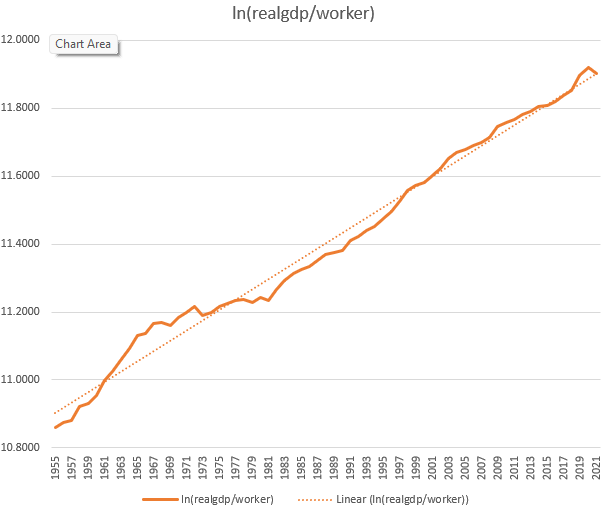
\includegraphics[width=0.6\textwidth]{graphs/lnrgdp_usa.png}
            \caption{Real GDP per Worker, US Economy
            \hyperlink{kaldor}{\beamergotobutton{Retour}}}
        \end{figure}
\end{frame}

\begin{frame}
    \frametitle{Kaldor's Stylized Facts}
    \hypertarget{capital}{} % Label for hyperlinks
    \framesubtitle{Accumulation de Capital}
        \begin{figure}
            \centering
            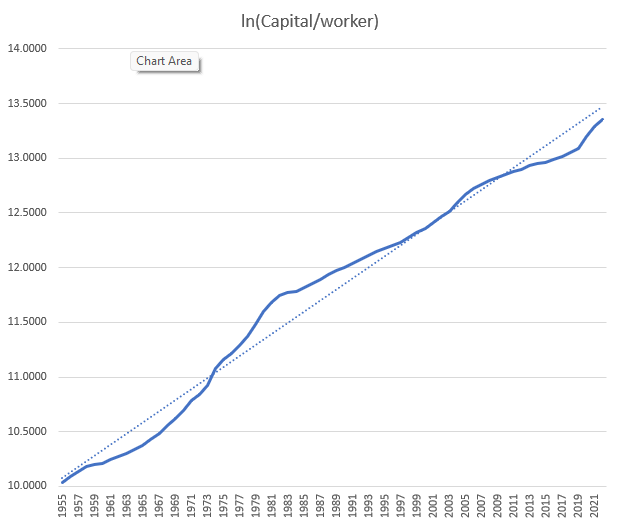
\includegraphics[width=0.6\textwidth]{graphs/lnkperworker_usa.png}
            \caption{Capital per Worker, US Economy
            \hyperlink{kaldor}{\beamergotobutton{Retour}}}
        \end{figure}
\end{frame}

\begin{frame}
    \frametitle{Kaldor's Stylized Facts}
    \hypertarget{capital_output_ratio}{} % Label for hyperlinks
    \framesubtitle{Ratio Capital-Production}
        \begin{figure}
            \centering
            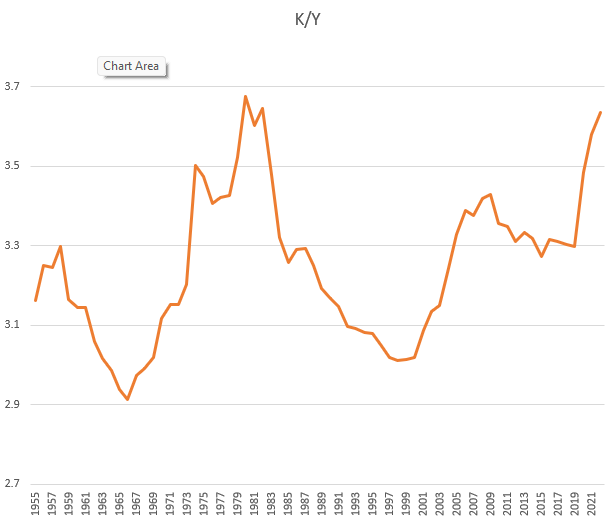
\includegraphics[width=0.55\textwidth]{graphs/kyratio_usa.png}
            \caption{\enquote*{Stability} of Capital-Output Ratio, US Economy
            \hyperlink{kaldor}{\beamergotobutton{Retour}}}
        \end{figure}
        
\end{frame}


\begin{frame}
    \frametitle{Kaldor's Stylized Facts}
    \hypertarget{income}{} % Label for hyperlinks
    \framesubtitle{Répartition du Revenu}
        \begin{figure}
            \centering
            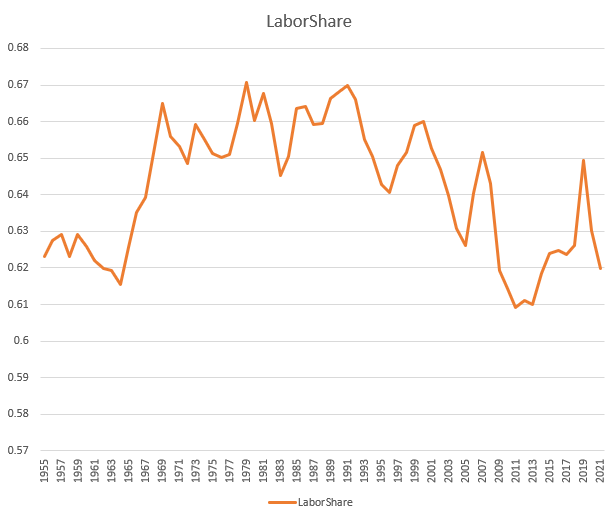
\includegraphics[width=0.6\textwidth]{graphs/labor_share.png}
            \caption{Labour Share of Income, US Economy
            \hyperlink{kaldor}{\beamergotobutton{Retour}}}
        \end{figure}
\end{frame}

\begin{frame}
    \frametitle{Kaldor's Stylized Facts}
    \hypertarget{return}{} % Label for hyperlinks
    \framesubtitle{Taux de Rendement}
        \begin{figure}
            \centering
            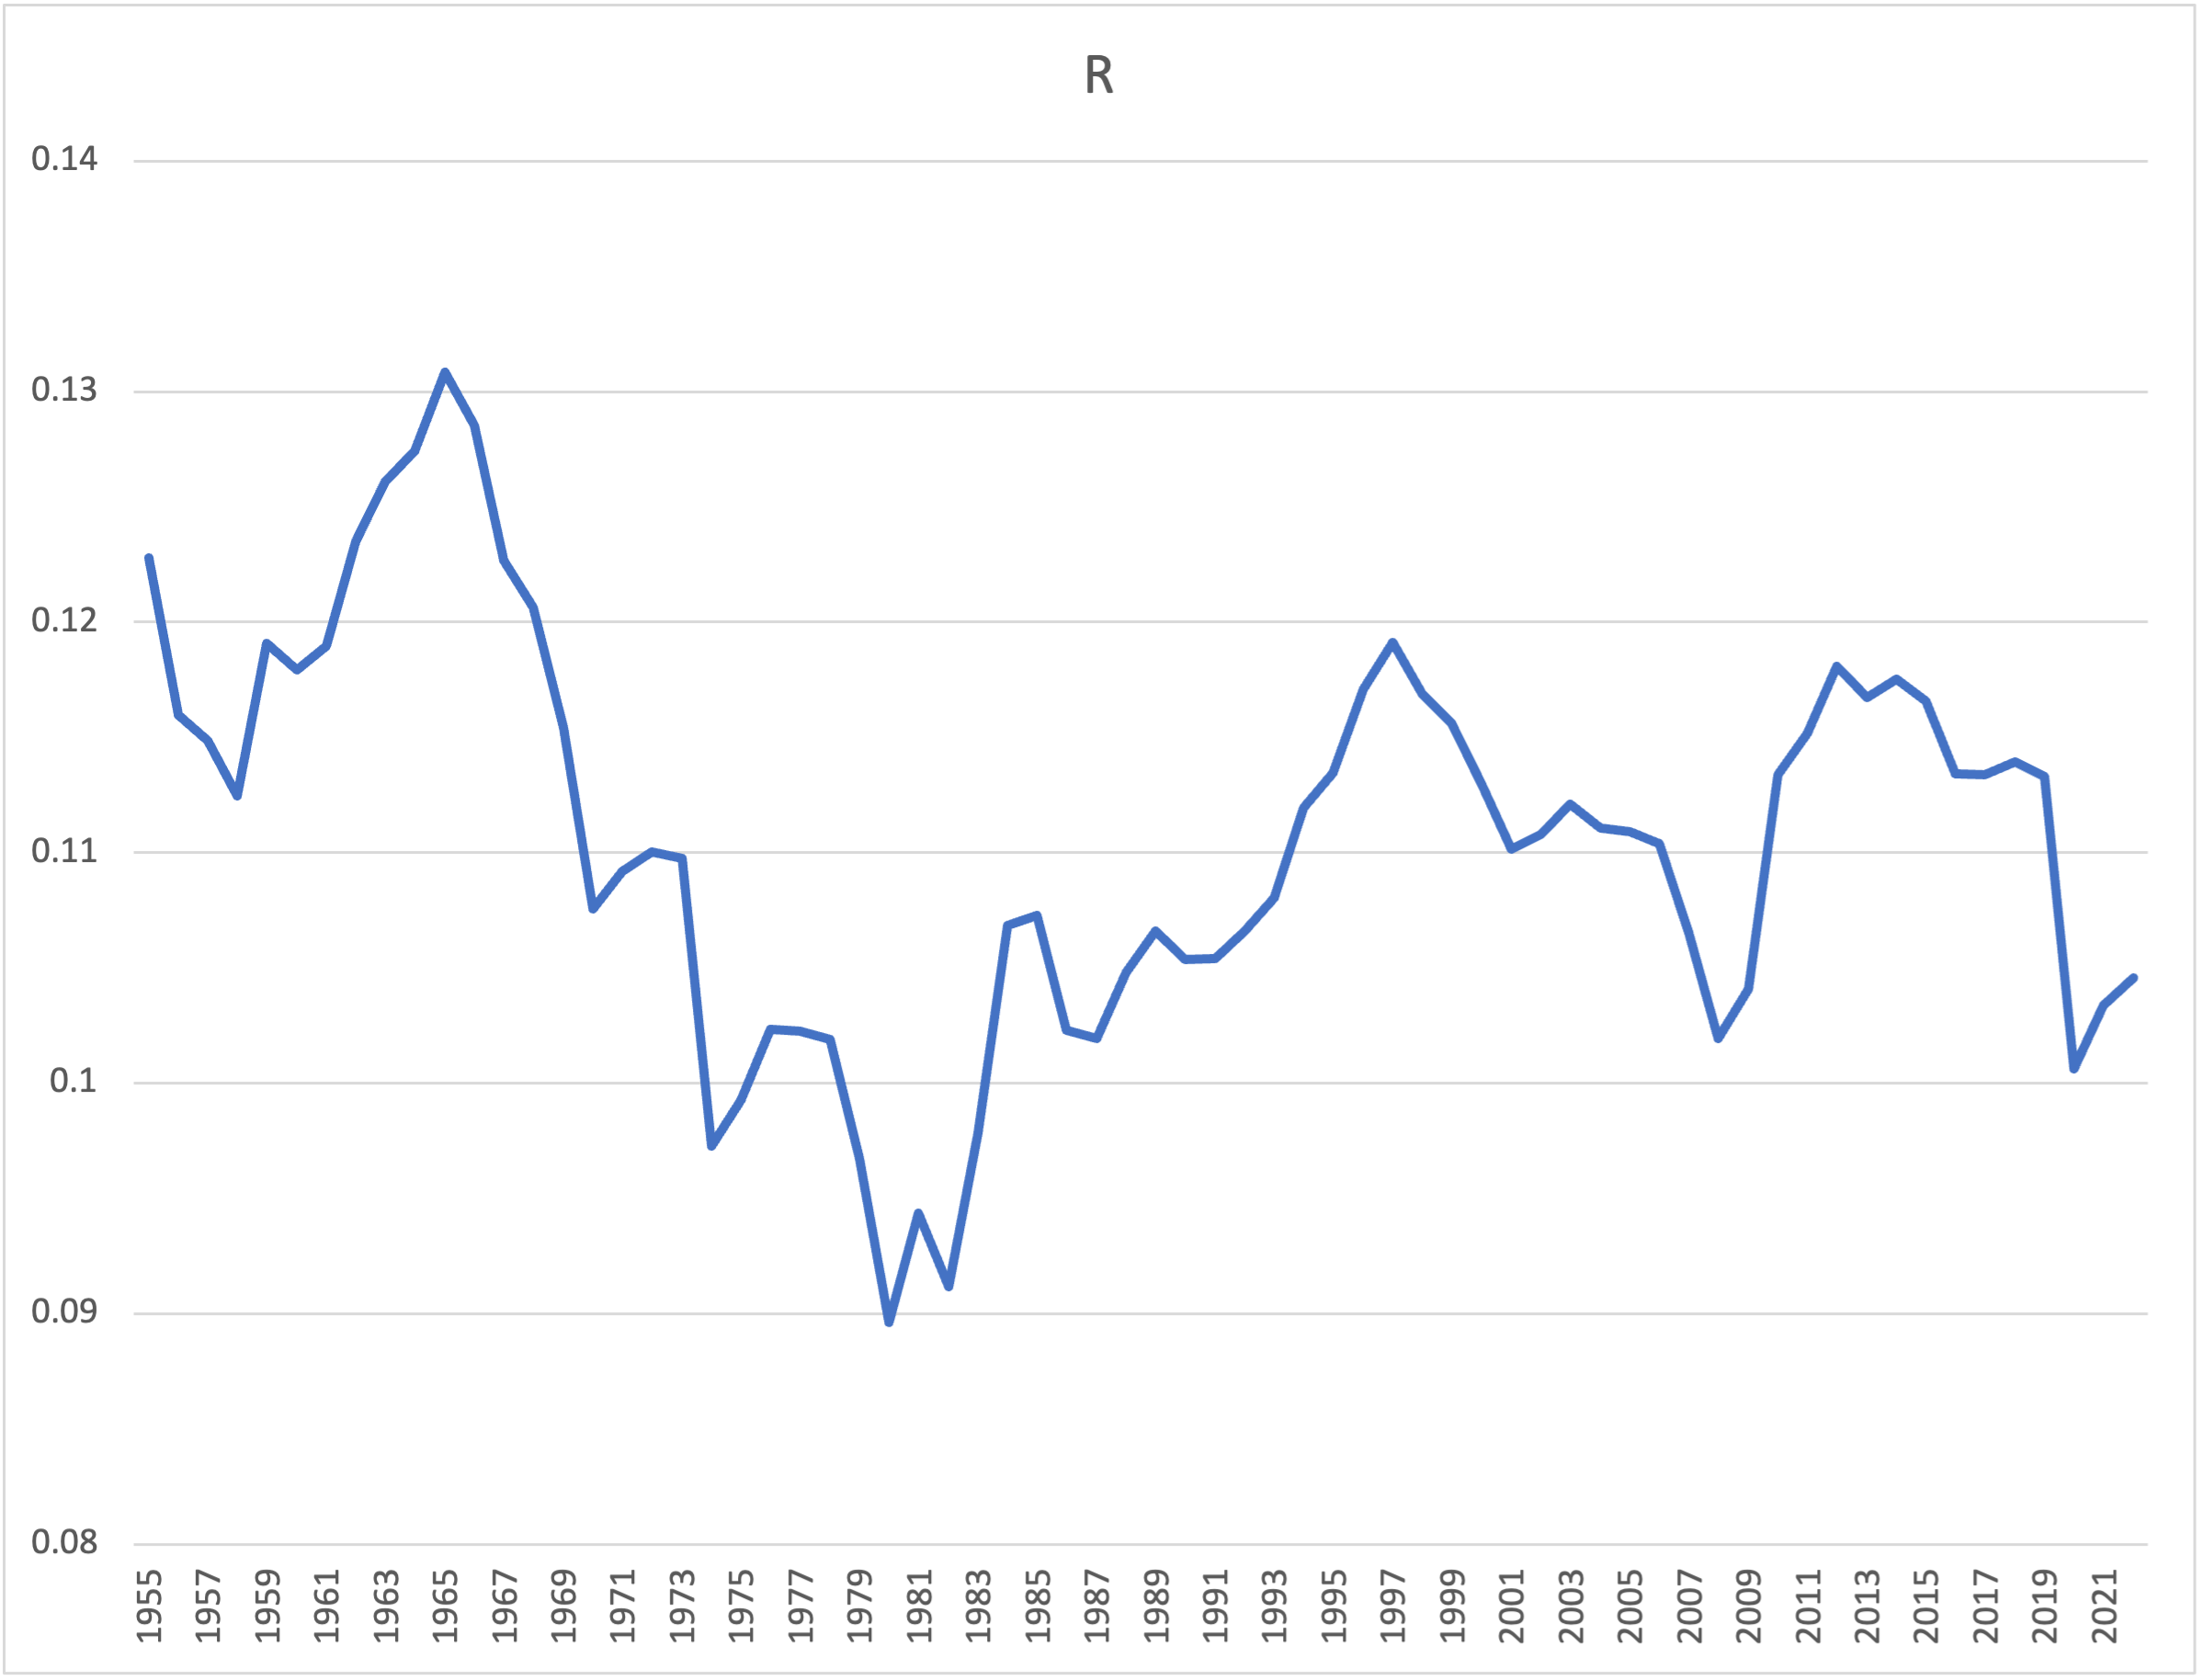
\includegraphics[width=0.6\textwidth]{graphs/r_usa.png}
            \caption{Return on Investment, US Economy}
        \end{figure}
\end{frame}


% \begin{frame}
%     \frametitle{Kaldor's Stylized Facts}
%     \hypertarget{return}{} % Label for hyperlinks
%     \framesubtitle{Taux de Rendement}
%         \begin{figure}
%             \centering
%             \includegraphics[width=0.8\textwidth]{graphs/}
%             \caption{Stability of Returns on Investment}
%         \end{figure}
% \end{frame}


\end{document}
